\begin{frame}
\frametitle{Problem 8 of Notes Chapter 5}
\begin{block}{Problem 8 of Notes Chapter 5}
Show that the sectional curvature of the sphere at all points is 1.
\end{block}
\end{frame}

\begin{frame}
\frametitle{Problem 8: Motivation}
We will derive the sectional curvature of a spherical surface of radius $R$. Note that while the calculations are straight-forward using the formulae for Christoffel symbols and Riemann tensor, the calculations are rather cumbersome and non-trivial. We aim to provide a detailed calculation of the various parameters, most of which may be skipped over due to want of time. The slides are however there to stay and will contain the detailed derivations.\\
\pause
Our basic layout is as follows:\\
\begin{figure}[!htb]
	\centering
   \begin{minipage}{0.8\textwidth}
     \centering
     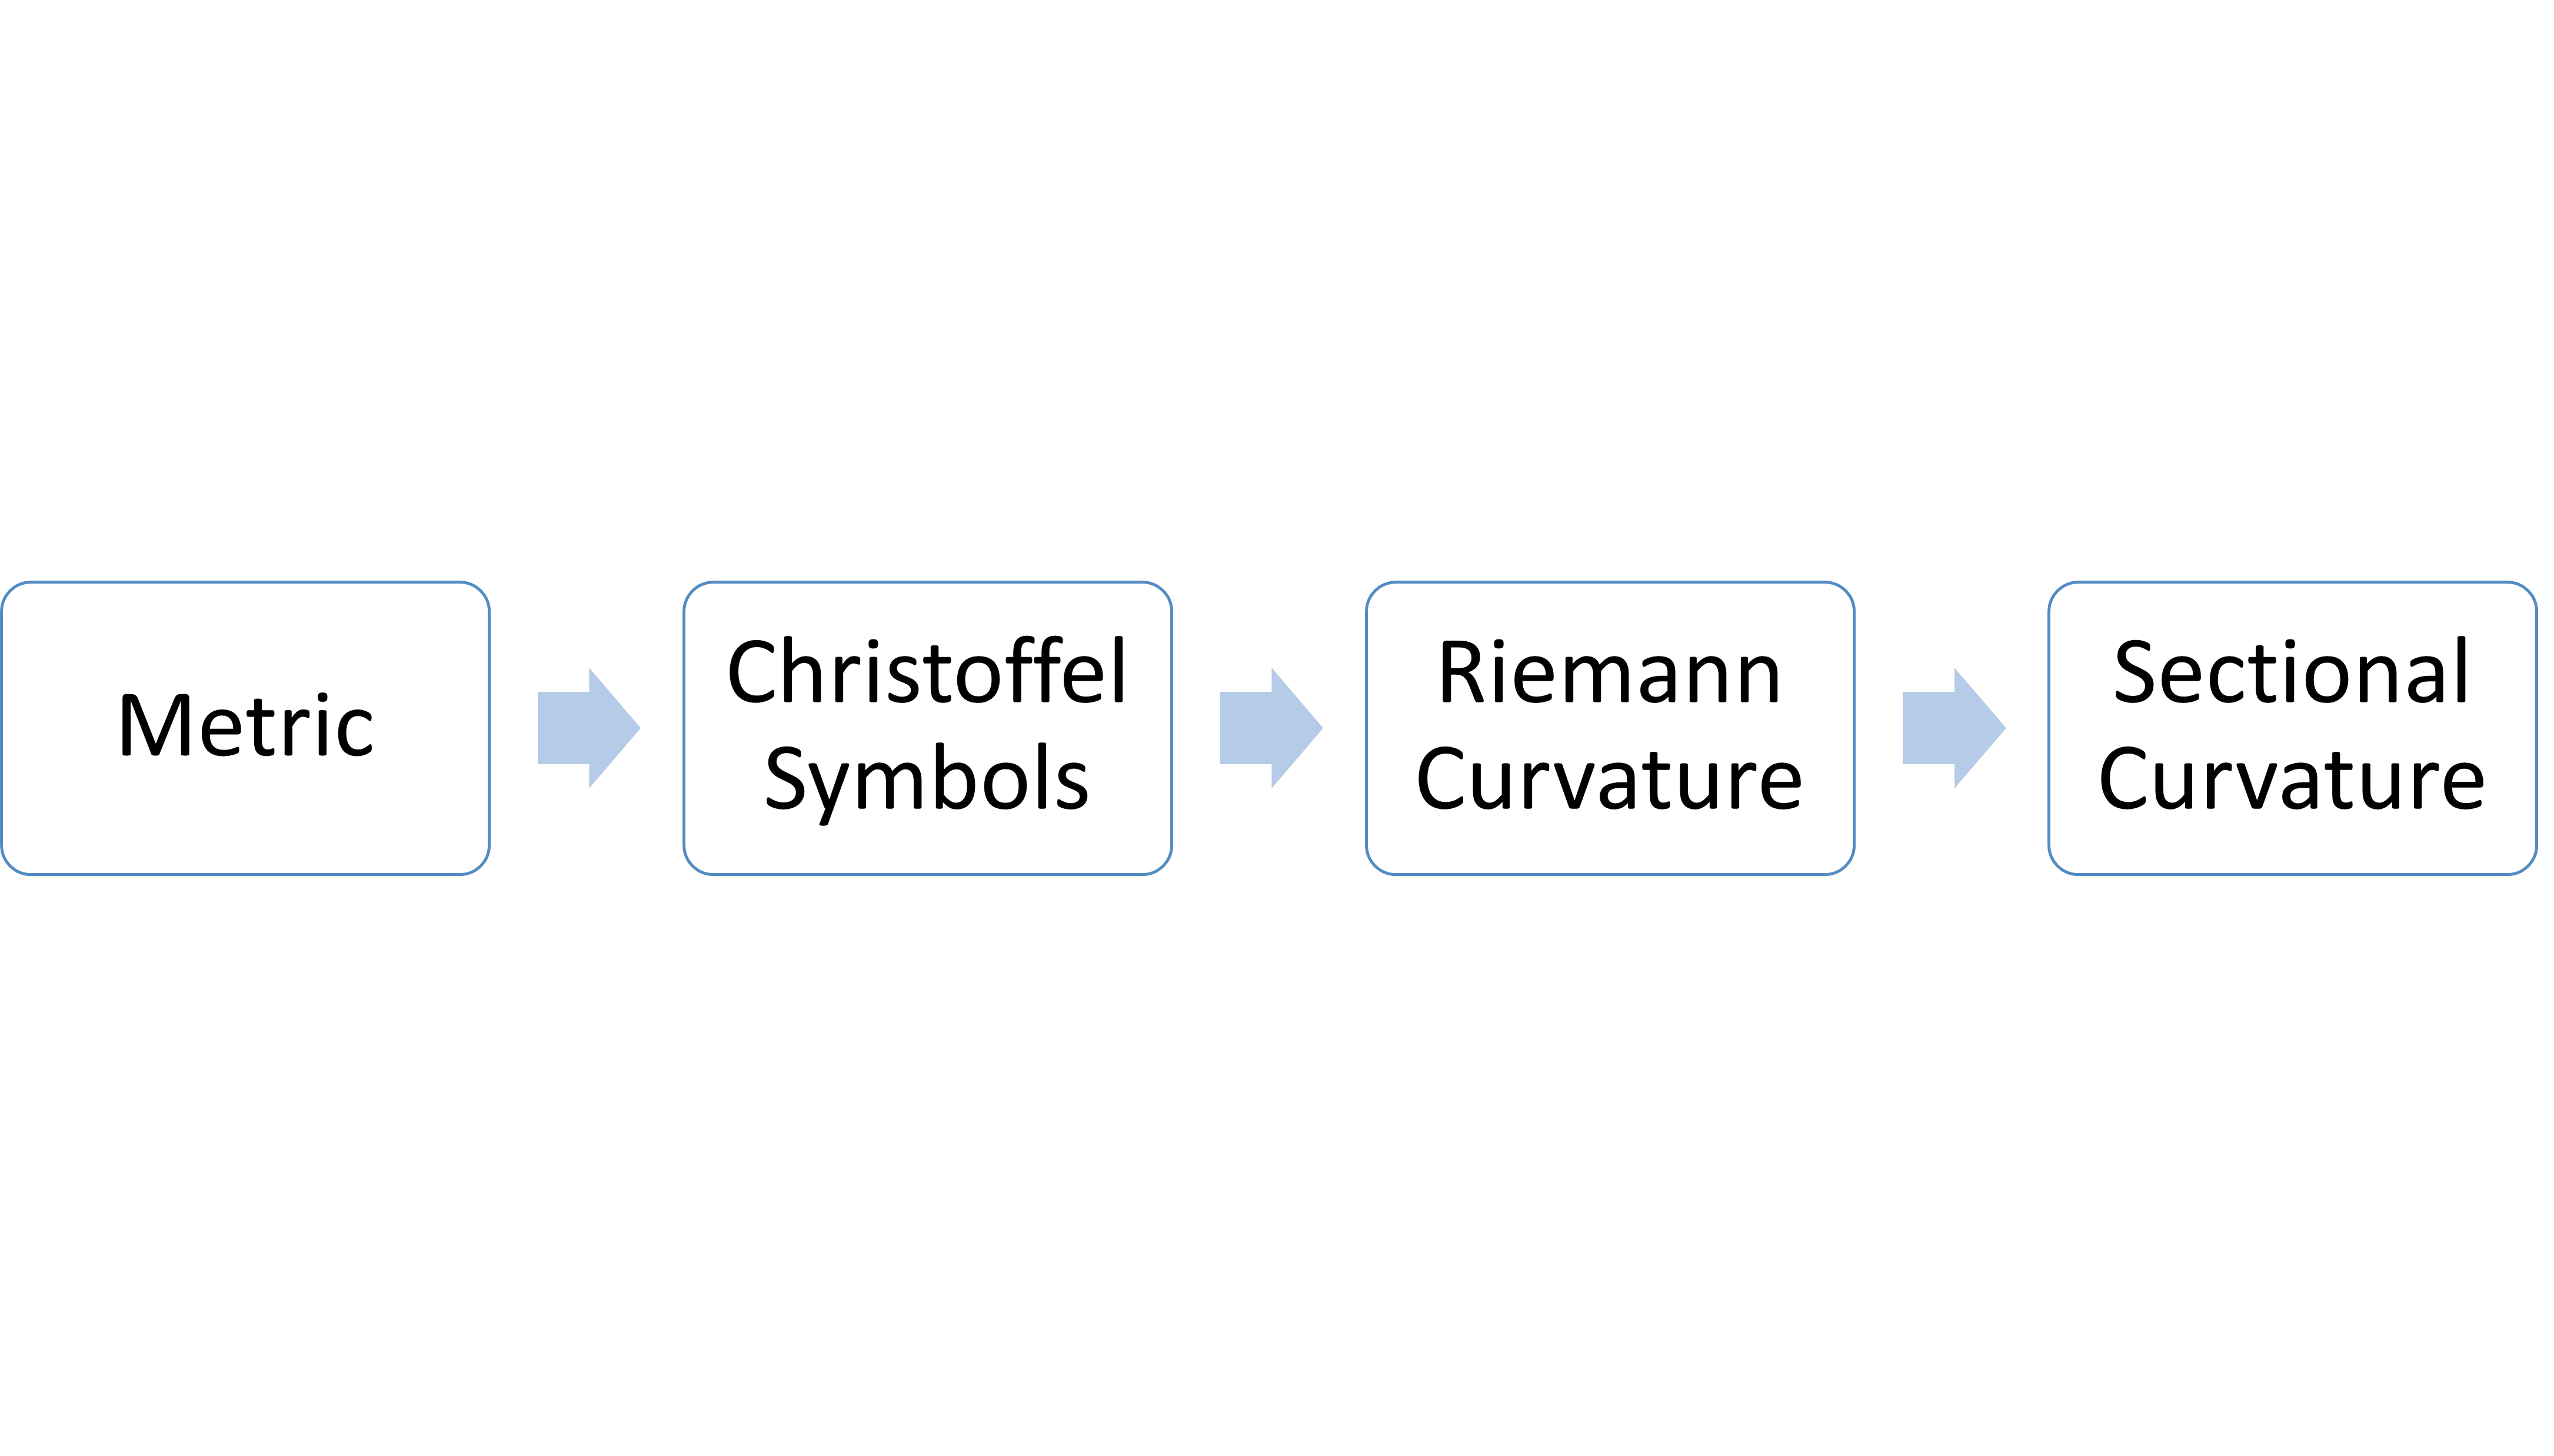
\includegraphics[width=0.5\linewidth]{img05.png}
     \caption{{Flowchart of our calculations}}
     \label{fig:05}
   \end{minipage}
\end{figure}
\end{frame}

\begin{frame}
\frametitle{Problem 8: Setting Up}
Some assumptions that we will make:
\begin{itemize}
\item We will assume the metric is given (this is one of the defining parameters of the manifold).\pause
\item We will follow the convention given in Do Carmo's book.\pause
\item We will use the formula for Christoffel symbols from metric.
\begin{align}
\label{christoffel symbols}
\Gamma^{\lambda}_{\mu\nu}=\bfrac{1}{2}g^{\lambda\alpha}(g_{\alpha\mu ,\nu}+g_{\alpha\nu ,\mu}-g_{\mu\nu ,\alpha})
\end{align}
where $\alpha$ is a dummy summation index.\pause
\item We will use the formula for Riemann curvature from Christoffel symbols (Lemma 5.5 of notes).
\begin{align}
\label{riemann curvature tensor}
R_{\lambda\mu\nu\sigma}=g_{\lambda\alpha}(\partial_\sigma\Gamma^{\alpha}_{\mu\nu}-\partial_\nu\Gamma^{\alpha}_{\mu\sigma}+\Gamma^{\alpha}_{\sigma\gamma}\Gamma^{\gamma}_{\mu\nu}-\Gamma^{\alpha}_{\nu\gamma}\Gamma^{\gamma}_{\mu\sigma})
\end{align}
where $\alpha$ and $\gamma$ are dummy summation indices.
\end{itemize}
\end{frame}

\begin{frame}
\frametitle{Problem 8: Specific Case of Sphere}
Note that out independent basis is formed by $(\theta,\phi)$ that span the surface of the sphere. The sphere is of radius $R$.\\ \pause
The distance metric is
\begin{align}
g=
\begin{pmatrix}
R^2 & 0\\
0 & R^2\sin^2\theta
\end{pmatrix}
\end{align}
i.e., $g_{\theta\theta}=R^2, g_{\theta\phi}=g_{\phi\theta}=0, g_{\phi\phi}=R^2\sin^2\theta$.\\ \pause
Calculating the inverse
\begin{align}
g^{-1}=
\begin{pmatrix}
\frac{1}{R^2} & 0\\
0 & \frac{1}{R^2\sin^2\theta}
\end{pmatrix}
\end{align}
i.e., $g^{\theta\theta}=\frac{1}{R^2}, g^{\theta\phi}=g^{\phi\theta}=0, g^{\phi\phi}=\frac{1}{R^2\sin^2\theta}$.\\
\end{frame}

\begin{frame}
\frametitle{Problem 8: Computing the Christoffel Symbols}
We will use equation \ref{christoffel symbols} to calculate the Christoffel symbols. We will also use the fact that the cross terms in the metric are zero.
\begin{align}
\Gamma^{\theta}_{\theta\theta}&=\bfrac{1}{2}g^{\theta\theta}(g_{\theta\theta ,\theta}+g_{\theta\theta ,\theta}-g_{\theta\theta ,\theta})=0\\
\Gamma^{\theta}_{\theta\phi}&=\bfrac{1}{2}g^{\theta\theta}(g_{\theta\theta ,\phi}+g_{\theta\phi ,\theta}-g_{\theta\phi ,\theta})=0\\
\Gamma^{\theta}_{\phi\theta}&=\bfrac{1}{2}g^{\theta\theta}(g_{\theta\phi ,\theta}+g_{\theta\theta ,\phi}-g_{\phi\theta ,\theta})=0\\
\Gamma^{\theta}_{\phi\phi}&=\bfrac{1}{2}g^{\theta\theta}(g_{\theta\phi ,\phi}+g_{\theta\phi ,\phi}-g_{\phi\phi ,\theta})=-\bfrac{1}{2}g^{\theta\theta}g_{\phi\phi ,\theta}=-\sin\theta\cos\theta
\end{align}
\end{frame}


\begin{frame}
\frametitle{Problem 8: Continuing the Computation of the Christoffel Symbols}
\begin{align}
\Gamma^{\phi}_{\theta\theta}&=\bfrac{1}{2}g^{\phi\phi}(g_{\phi\theta ,\theta}+g_{\theta\phi ,\theta}-g_{\theta\theta ,\phi})=0\\
\Gamma^{\phi}_{\theta\phi}&=\bfrac{1}{2}g^{\phi\phi}(g_{\theta\phi ,\phi}+g_{\phi\phi ,\theta}-g_{\theta\phi ,\phi})=\bfrac{1}{2}g^{\phi\phi}g_{\phi\phi ,\theta}=\bfrac{\cos\theta}{\sin\theta}\\
\Gamma^{\phi}_{\phi\theta}&=\bfrac{1}{2}g^{\phi\phi}(g_{\phi\phi ,\theta}+g_{\phi\theta ,\phi}-g_{\phi\theta ,\phi})=\bfrac{1}{2}g^{\phi\phi}g_{\phi\phi ,\theta}=\bfrac{\cos\theta}{\sin\theta}\\
\Gamma^{\phi}_{\phi\phi}&=\bfrac{1}{2}g^{\phi\phi}(g_{\phi\phi ,\phi}+g_{\phi\phi ,\phi}-g_{\phi\phi ,\phi})=0
\end{align}
\end{frame}

\begin{frame}
\frametitle{Problem 8: Riemann Curvature}
We shall calculate only $R_{\theta\phi\theta\phi}$ for calculating sectional curvature. It is straight-forwards but tedious to show that only the permutations of this tensor are non zero. We will use equation \ref{riemann curvature tensor}.
\begin{align}
R_{\theta\phi\theta\phi}&=g_{\theta\theta}(\partial_{\theta}\Gamma^{\theta}_{\phi\phi}-\partial_{\phi}\Gamma^{\theta}_{\phi\theta}+\Gamma^{\theta}_{\theta\theta}\Gamma^{\theta}_{\phi\phi}+\Gamma^{\theta}_{\theta\phi}\Gamma^{\phi}_{\phi\phi}-\Gamma^{\theta}_{\phi\theta}\Gamma^{\theta}_{\phi\theta}-\Gamma^{\theta}_{\phi\phi}\Gamma^{\phi}_{\phi\theta})\\
&=R^2(\sin^2\theta-\cos^2\theta-0+0+0-0-(-\sin\theta\cos\theta)(\bfrac{\cos\theta}{\sin\theta}))\\
&=R^2\sin^2\theta
\end{align}
\end{frame}

\begin{frame}
\frametitle{Problem 8: Sectional Curvature}
So far we have
\begin{align}
R_{\theta\phi\theta\phi}=R^2\sin^2\theta
\end{align}
Also, we have the formula for sectional curvature
\begin{align}
K(v,w)=\bfrac{\inner{R(v,w)w,v)}}{\abs{v\wedge w}^2}=\bfrac{R_{vwvw}}{\det(g)}
\end{align}
Hence, we get the sectional curvature of the sphere to be
\begin{align}
K(\theta,\phi)=\bfrac{R_{\theta\phi\theta\phi}}{\det(g)}=\bfrac{R^2\sin^2\theta}{R^4\sin^2\theta}=\bfrac{1}{R^2}
\end{align}
\end{frame}

\begin{frame}
\frametitle{Problem 8: QED}
Thus, for a unit sphere, curvature is constant ($=1$) at all points, irrespective of the values of $\theta$, $\phi$.\\ \pause
\begin{block}{Bonus}
What surface has constant negative curvature (say, -1)?
\end{block}

\end{frame}

